\documentclass{article}

\usepackage{enumerate}
\usepackage{amssymb}
\usepackage{amsmath}
\usepackage{algorithm}
\usepackage{physics}
\usepackage{listings}
\usepackage[noend]{algpseudocode}
\usepackage{graphicx}

\graphicspath{ {./} }

\topmargin=-0.45in
\evensidemargin=0in
\oddsidemargin=0in
\textwidth=6.5in
\textheight=9.0in
\headsep=0.25in

\title{Chem 195: Problem Set 7}
\author{Michael Stephen Chen}


\begin{document}
\maketitle
\pagebreak

\section*{Problem 1}

\begin{center}
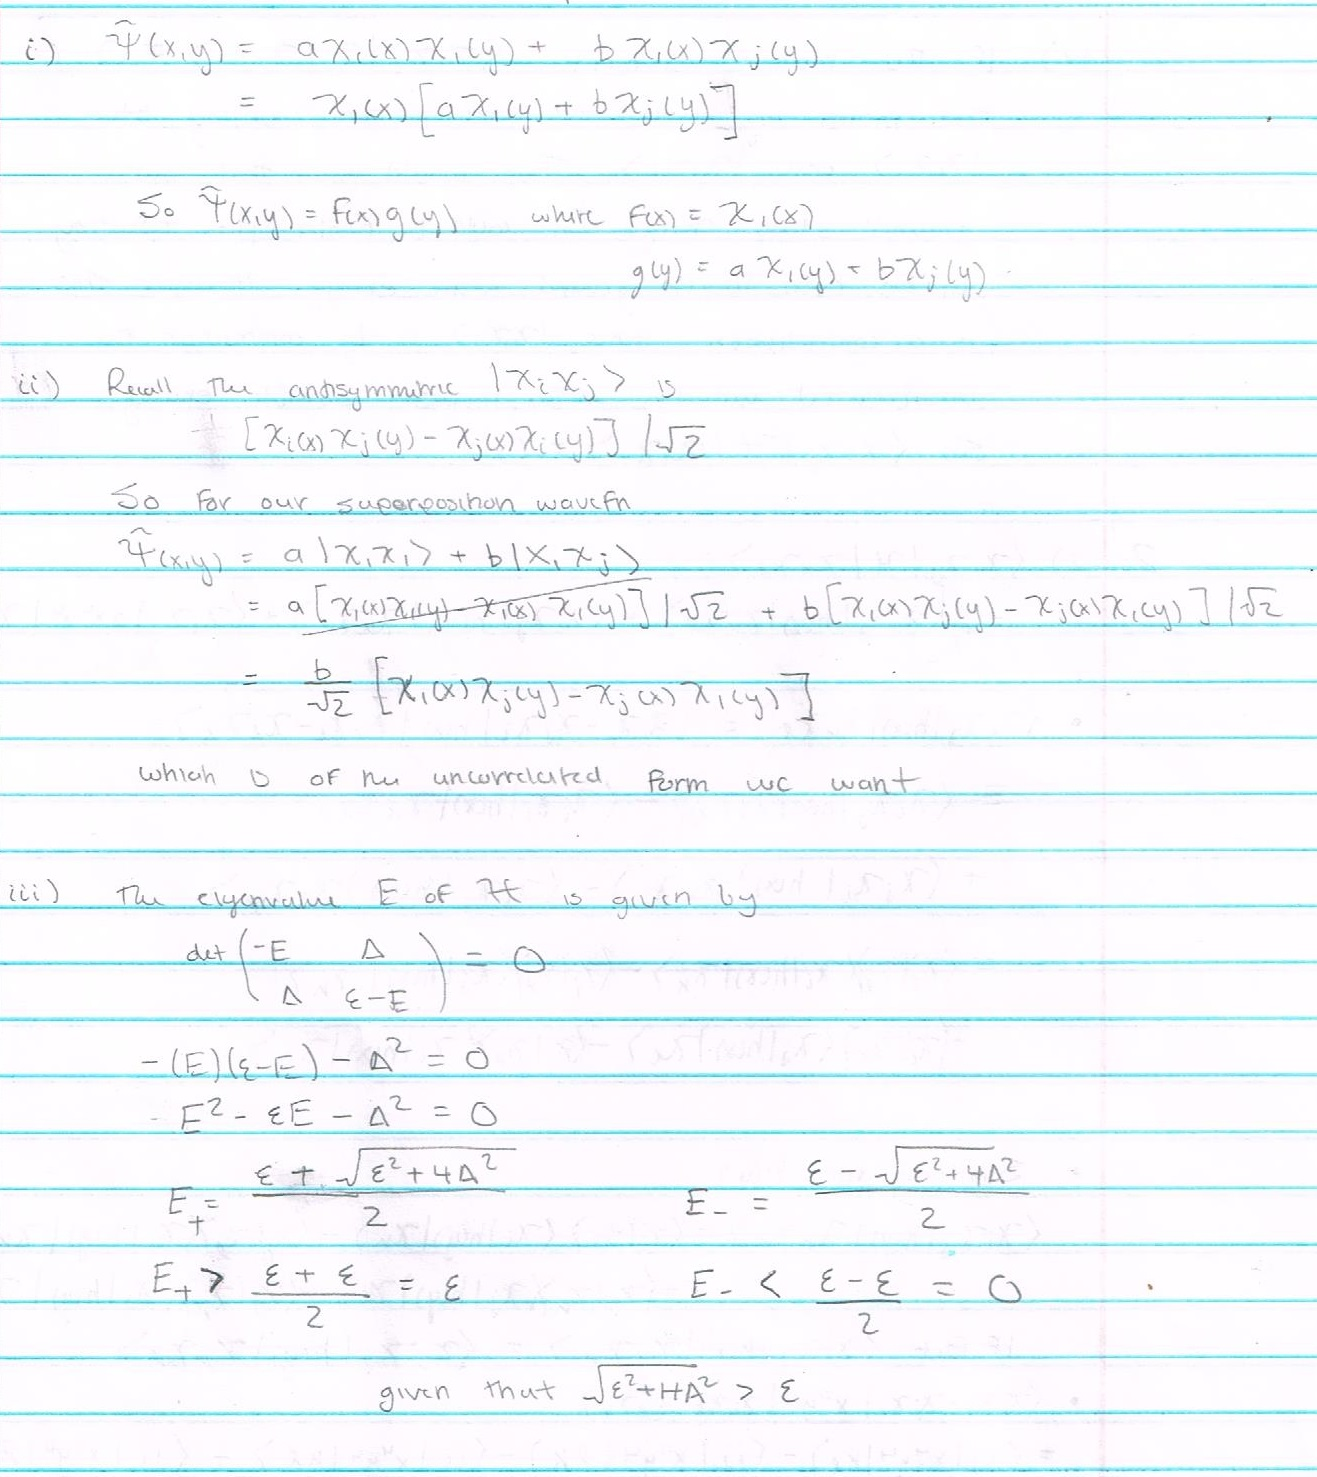
\includegraphics[scale=0.75]{prob1_1}\\
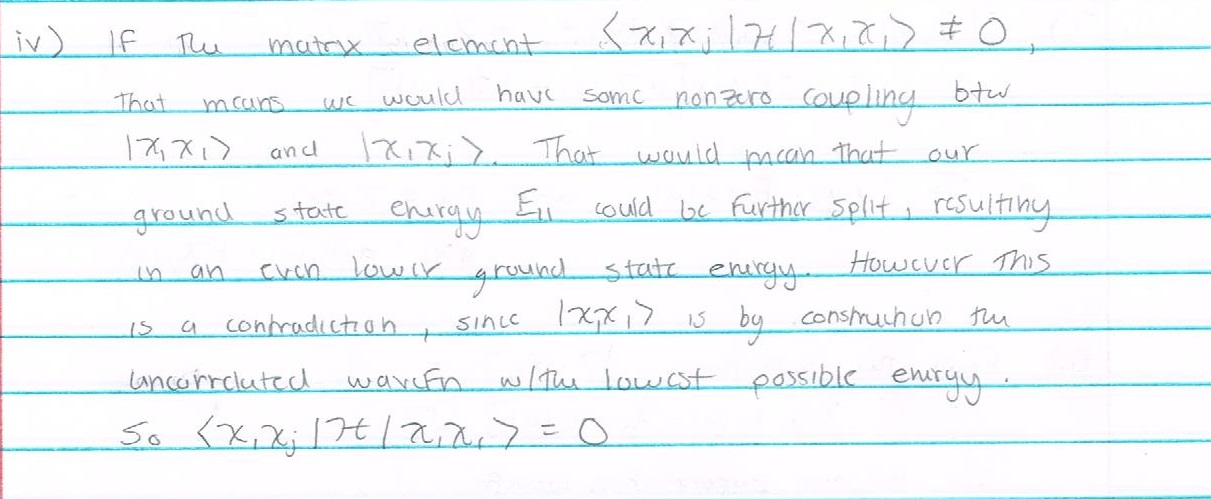
\includegraphics[scale=0.75]{prob1_2}
\end{center}

\section*{Problem 2}

\begin{center}
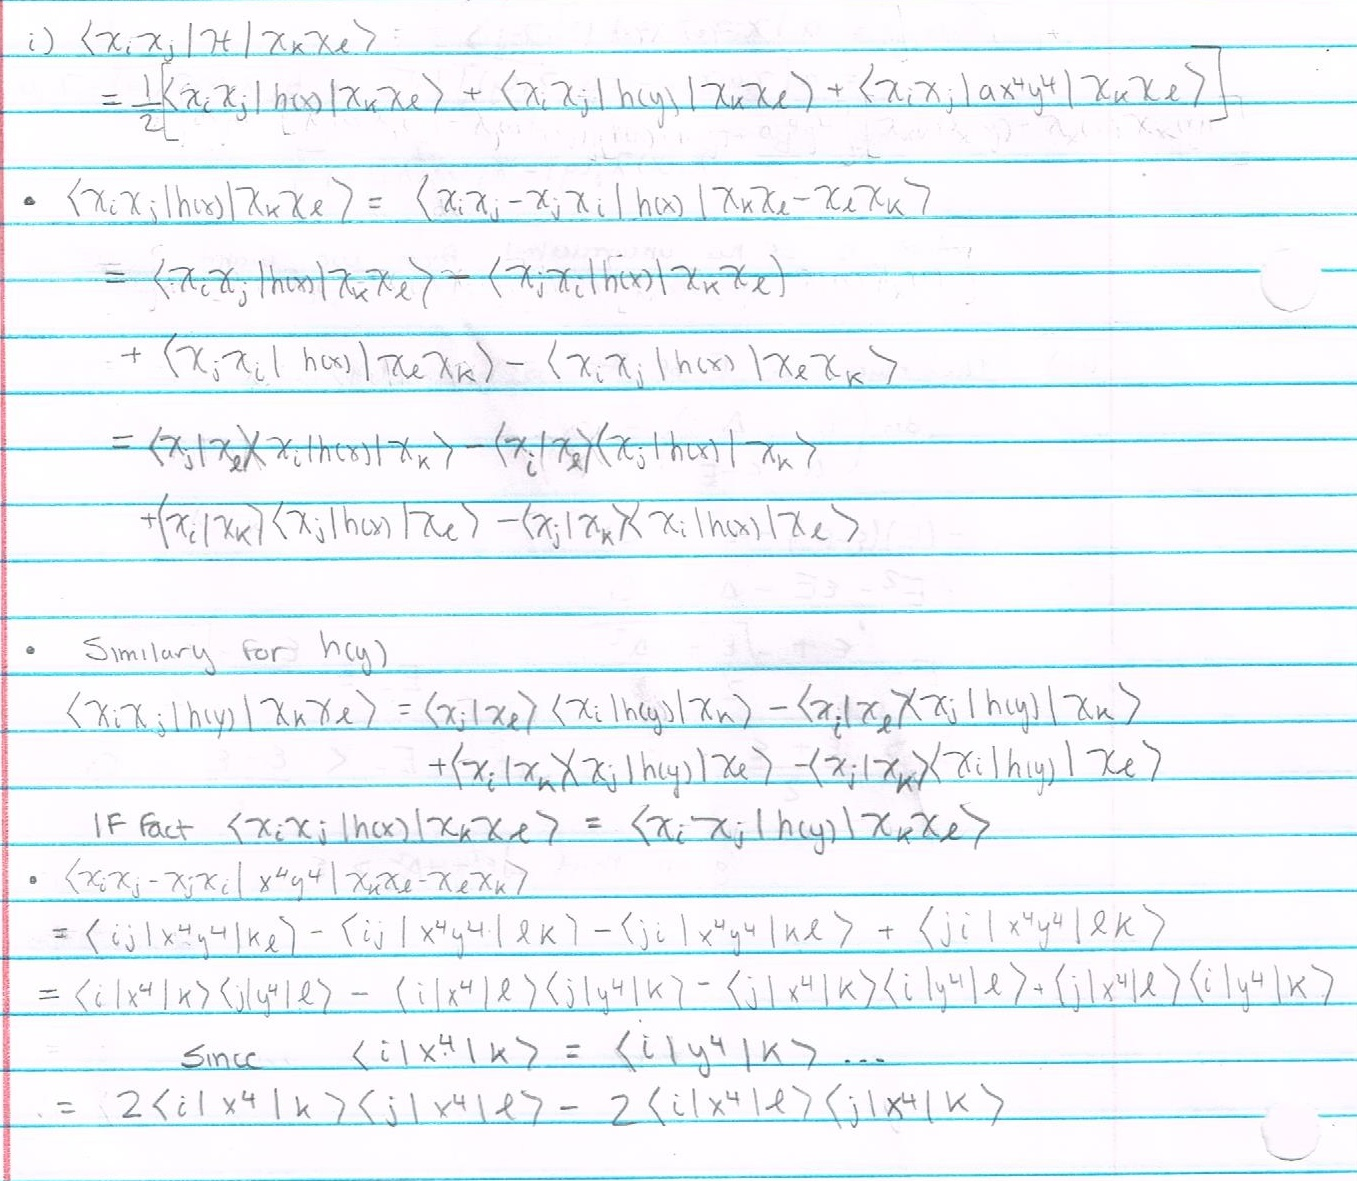
\includegraphics[scale=0.75]{prob2_1}\\
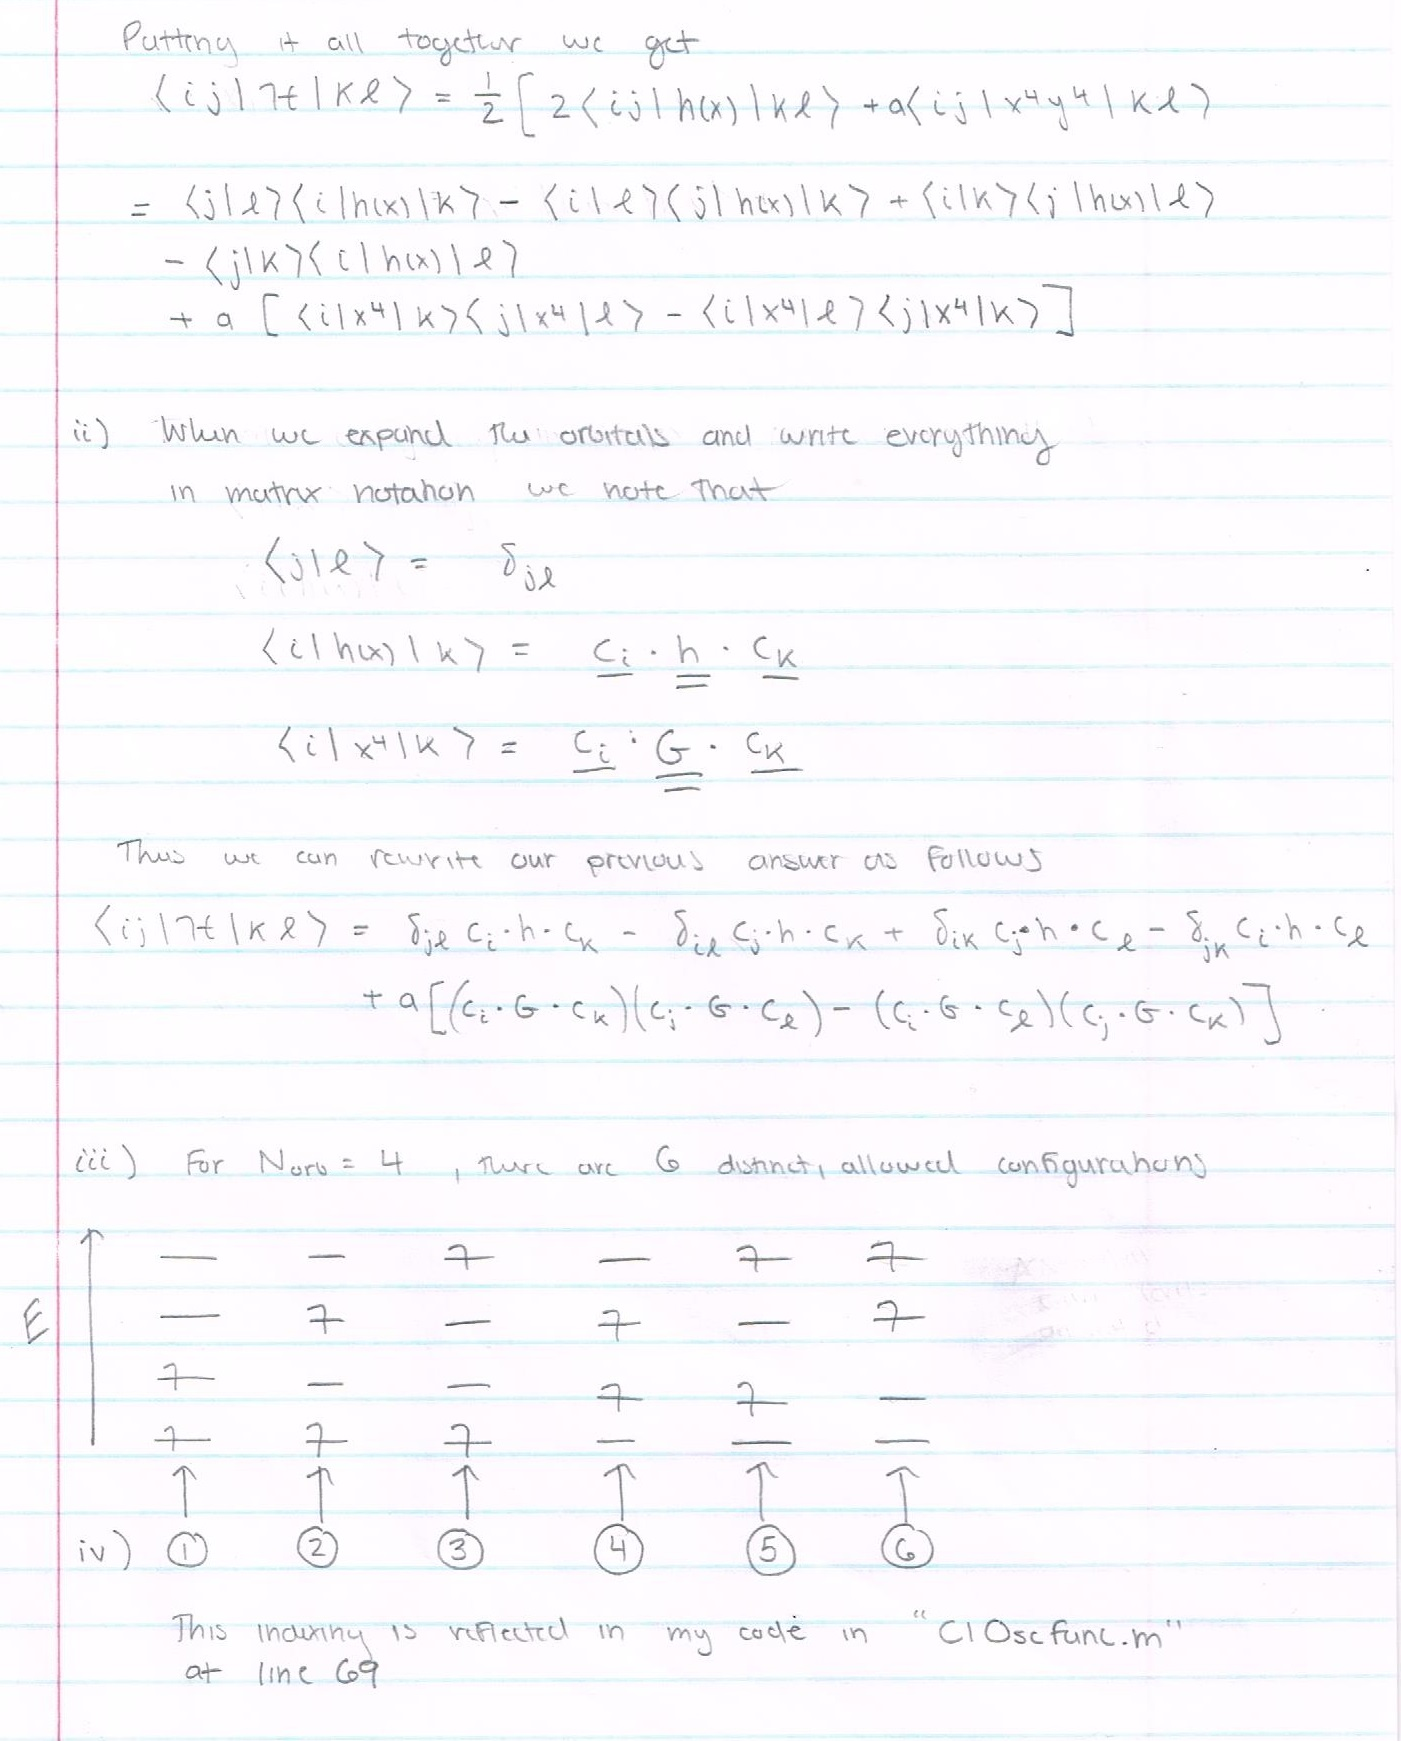
\includegraphics[scale=0.75]{prob2_2}
\end{center}
\pagebreak

For $N_{orb} = 4$, the CI method gives us a ground state energy of $2.4870 Hartrees$ for an anharmonic factor of $a = 1.0$. Below is a plot depicting ground state energies as a function of the anharmonic factor $a \in \left[ 0, 10\right]$:
\begin{center}
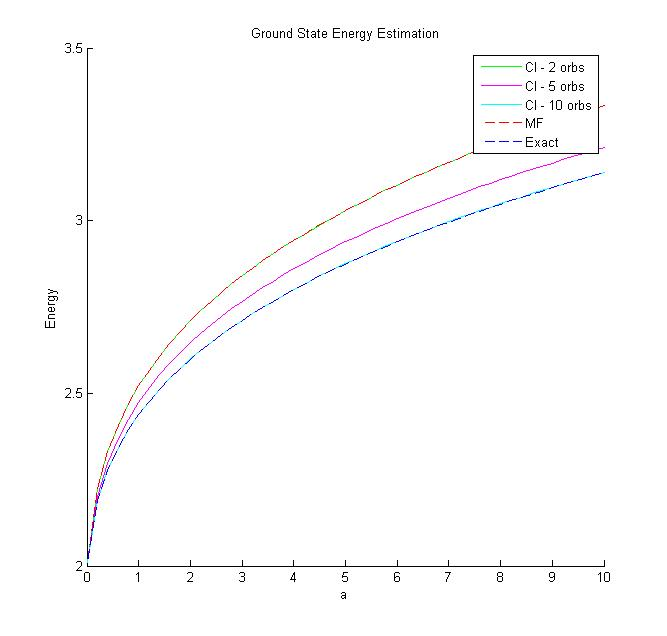
\includegraphics[scale=0.5]{prob2vi}
\end{center}

From the plot we see that the CI results when we use only two orbitals are exactly the same as the mean field results. This is unsurprising because when $N_{orb}=2$ for our CI method, that means that there is only one configuration that is possible (i.e. the symmetry-constrained mean field ground state).

We also see that as we increase the number of orbitals for our CI calculations, we approach the ``exact'' solution. In fact when by the time we reach $N_{orb}=10$ the ground state energies are essentially the same as the ``exact'' values, attesting to the accuracy of the CI method.

\end{document}
